\documentclass[12pt, a4paper, oneside]{ctexart}
\usepackage{amsmath, amsthm, amssymb, bm, color, graphicx, geometry, hyperref, mathrsfs,extarrows, braket, booktabs, array}

\linespread{1.5}
%\geometry{left=2.54cm,right=2.54cm,top=3.18cm,bottom=3.18cm}
\geometry{left=1.84cm,right=1.84cm,top=2.18cm,bottom=2.18cm}
\newenvironment{problem}{\par\noindent\textbf{题目. }}{\bigskip\par}
\newenvironment{solution}{\par\noindent\textbf{解答. }}{\bigskip\par}
\newenvironment{note}{\par\noindent\textbf{注记. }}{\bigskip\par}

% 基本信息
\newcommand{\RQ}{\today} % 日期
\newcommand{\km}{概率论} % 科目
\newcommand{\bj}{强基数学002} % 班级
\newcommand{\xm}{吴天阳} % 姓名
\newcommand{\xh}{2204210460} % 学号

\begin{document}

%\pagestyle{empty}
\pagestyle{plain}
\vspace*{-15ex}
\centerline{\begin{tabular}{*5{c}}
    \parbox[t]{0.25\linewidth}{\begin{center}\textbf{日期}\\ \large \textcolor{blue}{\RQ}\end{center}} 
    & \parbox[t]{0.2\linewidth}{\begin{center}\textbf{科目}\\ \large \textcolor{blue}{\km}\end{center}}
    & \parbox[t]{0.2\linewidth}{\begin{center}\textbf{班级}\\ \large \textcolor{blue}{\bj}\end{center}}
    & \parbox[t]{0.1\linewidth}{\begin{center}\textbf{姓名}\\ \large \textcolor{blue}{\xm}\end{center}}
    & \parbox[t]{0.15\linewidth}{\begin{center}\textbf{学号}\\ \large \textcolor{blue}{\xh}\end{center}} \\ \hline
\end{tabular}}
\vspace*{4ex}

\paragraph{习题 3.1}
\paragraph{1.} 设 $A$ 和$B$是同一个概率空间中的两个随机事件。证明:(1) $I_{A\triangle B} = (I_A-I_B)^2$; (2) $I_{A\triangle B} = |I_A-I_B|$; (3) $I_{A\cup B} = \max\{I_A,I_B\}$; (4) $I_{A\cap B}=\min\{I_A, I_B\}$; (5) $I_{A\cap B} = I_A\cdot I_B$。
\begin{proof}
    (1) \begin{equation*}
        \begin{aligned}
            I_{A\triangle B} =&\ I_{A^cB\cup AB^c} = I_{A^cB}+I_{AB^c}=I_{A^c}I_B+I_AI_{B^c}=(1-I_A)I_B+I_A(1-I_B)\\
            =&\ I_A+I_B-2I_AI_B = I_A^2+I_B^2-2I_AI_B=(I_A-I_B)^2
        \end{aligned}
    \end{equation*}

    (2)\begin{equation*}
        \begin{aligned}
            I_{A\triangle B} = (I_A-I_B)^2\xlongequal{\text{由于}(I_A-I_B)^2\text{的值域为}\{0,1\}}|I_A-I_B|
        \end{aligned}
    \end{equation*}

    (3)\begin{equation*}
        \begin{aligned}
            &\ \omega\in A\lor \omega\in B\iff I_A(\omega) = I_B(\omega) = 1\iff I_{A\cup B}(\omega) = \max\{I_A(\omega),I_B(\omega)\} = 1\\
            &\ \omega\notin A\land \omega\notin B\iff I_A(\omega) = I_B(\omega) = 0\iff I_{A\cup B}(\omega) = \max\{I_A(\omega),I_B(\omega)\} = 0\\
            \Rightarrow &\ I_{A\cup B} = \max\{I_A,I_B\}
        \end{aligned}
    \end{equation*}

    (4)\begin{equation*}
        \begin{aligned}
            &\ \omega\in A\land \omega\in B\iff I_A(\omega) =  I_B(\omega) = 1\iff I_{A\cap B}(\omega) = \min\{I_A(\omega),I_B(\omega)\} = 1\\
            &\ \omega\notin A\lor \omega\notin B\iff I_A(\omega) = I_B(\omega) = 0\iff I_{A\cap B}(\omega) = \min\{I_A(\omega),I_B(\omega)\} = 0\\
            \Rightarrow &\ I_{A\cap B} = \min\{I_A,I_B\}
        \end{aligned}
    \end{equation*}
    
    (5)\begin{equation*}
        \begin{aligned}
            &\ \omega\in A\land \omega\in B\iff I_A(\omega) = I_B(\omega) = 1\iff I_{A\cap B}(\omega) = I_A(\omega)\cdot I_B(\omega) = 1\\
            &\ \omega\notin A\lor \omega\notin B\iff I_A(\omega) = I_B(\omega) = 0\iff I_{A\cap B}(\omega) = I_A(\omega)\cdot I_B(\omega) = 0\\
            \Rightarrow &\ I_{A\cap B} = I_A\cdot I_B
        \end{aligned}
    \end{equation*}
\end{proof}
\paragraph{2.}$C$应取何值才能使下列函数称为概率分布:
\begin{equation*}
    (1)\ f(k) = \frac{C}{N},\quad k=1,2,\cdots,N;\quad\quad(2)\ f(k)=C\frac{\lambda^k}{k!},\quad k=1,2,\cdots,\quad \lambda > 0.
\end{equation*}
\begin{solution}
    (1) \begin{equation*}
        \begin{aligned}
            \sum_{k=1}^Nf(k) = \sum_{k=1}^N\frac{C}{N} = C = 1
        \end{aligned}
    \end{equation*}
    
    (2)\begin{equation*}
        \begin{aligned}
            &\sum_{k=1}^{\infty}f(k) = C\sum_{k=1}^{\infty}\frac{\lambda^k}{k!} = C(e^\lambda - 1) = 1\\
            \Rightarrow &\ C=  \frac{1}{e^\lambda - 1}
        \end{aligned}
    \end{equation*}
\end{solution}
\paragraph{5.}若对每个$n\geqslant 1$,$X_n$都是随机变量,证明
\begin{equation*}
    \sup_{n\geqslant 1}X_n,\quad \inf_{n\geqslant 1}X_n,\quad \limsup_{n\rightarrow\infty}X_n,\quad \liminf_{n\rightarrow\infty}X_n
\end{equation*}
均为随机变量。
\begin{proof}
    $\forall x\in \mathbb{R}$,则
    \begin{equation*}
        \sup_{n\geqslant 1}X_n\leqslant x = \left\{\omega \in \mathscr{F}:\left(\sup_{n\geqslant1}X_n(\omega)\right)\leqslant x\right\} = \left\{\omega\in\mathscr{F}:x\in \sup_{n\geqslant 1}x_n(\omega)\right\}
    \end{equation*}
    所以
    \begin{equation*}
        \begin{aligned}
            &\ \omega\in\sup_{n\geqslant 1}X_n\leqslant x\iff \sup_{n\geqslant 1}X_n(\omega)\leqslant x\iff x\in \sup_{n\geqslant 1}X_n(\omega)\\
            \iff&\ x_1(\omega)\leqslant x\land x_2(\omega)\leqslant x\land\cdots\land x_n(\omega)\leqslant x\land\cdots\\
            \iff&\ \omega\in\bigcap_{n=1}^{\infty}\{X_n\leqslant x\}\\
            \Rightarrow&\ \sup_{n\geqslant 1}X_n\leqslant x  = \bigcap_{n=1}^{\infty}\{X_n\leqslant x\}
        \end{aligned}
    \end{equation*}
    由于$\{X_n\leqslant x\}\subset \mathscr{F}$,且$\mathscr{F}$为一个$\sigma$-域,其子集的交仍为其子集,所以$\bigcap\limits_{n=1}^\infty \{X_n\leqslant x\}\subset \mathscr{F}$为一个事件,故$\sup\limits_{n\geqslant 1}X_n$为随机变量。同理可得,$\inf\limits_{n\geqslant 1}X_n$也为随机变量。

    \begin{equation*}
        \limsup_{n\rightarrow\infty}x_n=\inf_{n\geqslant 1}\left\{\sup_{m\geqslant n}X_m\right\}
    \end{equation*}
    由上述证明可知,$Y_n=\displaystyle\sup_{m\geqslant n}X_m$为随机事件,则$\displaystyle\inf_{n\geqslant 1}Y_n=\limsup_{n\rightarrow\infty}x_n$也为随机变量。同理可得,$\displaystyle\liminf_{n\rightarrow\infty}x_n$也为随机变量。
\end{proof}
\paragraph{6.}袋中有$5$个同型号的小球,编号为$1,2,3,4,5$,从袋中任取三个球,用$X$表示取出的球中的最大编号,求$X$的分布律。
\begin{solution}
    设样本空间$|\Omega|$为取出三种球的全部情况,则$|\Omega|  = \binom{5}{3}=10$,则
    \begin{equation*}
        \begin{aligned}
            &\textbf{P}(X = 3) = \frac{1}{10},\quad\textbf{P}(X = 4) = \frac{3}{10},\quad\textbf{P}(X = 5) = \frac{6}{10}=\frac{3}{5}\\
        \end{aligned}
    \end{equation*}
    所以$X$的分布律可以记为
    \begin{equation*}
        \left(\begin{matrix}
            3&4&5\\
            \frac{1}{10}&\frac{3}{10}&\frac{3}{5}
        \end{matrix}\right)
    \end{equation*}
\end{solution}
\paragraph{9.}从$1,2,\cdots,10$十个数中无放回随机地取出五个数字,将这五个数字按由小到大的顺序排成一行:$X_1<X_2<X_3<X_4<X_5$。求$X_1$和$X_3$的分布律。如果取数是有放回的(这时$X_1\leqslant X_2\leqslant X_3\leqslant X_4\leqslant X_5$,$X_1,X_3$和$X_5$的分布律又个为什么?
\begin{solution}无放回时
    \begin{equation*}
        \begin{aligned}
            &X_1\text{的分布律:}\quad\left(\begin{matrix}
                1&2&3&4&5&6\\
                \dfrac{\binom{9}{4}}{\binom{10}{5}}&\dfrac{\binom{8}{4}}{\binom{10}{5}}&\dfrac{\binom{7}{4}}{\binom{10}{5}}&\dfrac{\binom{6}{4}}{\binom{10}{5}}&\dfrac{\binom{5}{4}}{\binom{10}{5}}&\dfrac{\binom{4}{4}}{\binom{10}{5}}
            \end{matrix}\right)\\
            &X_3\text{的分布律:}\quad\left(\begin{matrix}
                3&4&5&6&7&8\\
                \dfrac{\binom{2}{2}\binom{7}{2}}{\binom{10}{5}}&\dfrac{\binom{3}{2}\binom{6}{2}}{\binom{10}{5}}&\dfrac{\binom{4}{2}\binom{5}{2}}{\binom{10}{5}}&\dfrac{\binom{5}{2}\binom{4}{2}}{\binom{10}{5}}&\dfrac{\binom{6}{2}\binom{3}{2}}{\binom{10}{5}}&\dfrac{\binom{7}{2}\binom{2}{2}}{\binom{10}{5}}
            \end{matrix}\right)\\
        \end{aligned}
    \end{equation*}

    有放回时较为复杂。设共有$i$个数:$1,2,\cdots, i$有放回地取出$j$个,从小到大排序排成一行:$X_1\leqslant X_2\leqslant \cdots\leqslant X_i$,将$X_1X_2\cdots X_i$的所有可能情况记为事件$B_{ij}$,其中$X_i=1$的情况记为事件$A_{ij}$。不难发现
    \begin{equation*}
        B_{ij} = A_{1j}+A_{2j} +\cdots +A_{ij}
    \end{equation*}
    下面求解$A_{ij}$,我们可以将$A_{ij}$分解成两个不交集合的并:$A_{i-1,j}+A_{i,j-1}$,因为可以做出如下构造:
    
    $\forall Y_1Y_2\cdots Y_j\in A_{i-1,j}$,有$X_1(Y_1+1)(Y_2+1)\cdots(Y_{j-1}+1)\in A_{ij}$,

    $\forall X_1X_2\cdots X_{j-1}\in A_{i, j-1}$,有$X_1X_1X_2\cdots X_{j-1}\in A_{ij}$,容易证明$A_{ij}$中的元素一定可由这两种方法之一生成,故$A_{ij} = A_{i-1,j} + A_{i, j-1}$,于是$|A_{ij}| = |A_{i-1,j}|+|A_{i,j-1}|$,通过制表找规律:

    \centerline{
        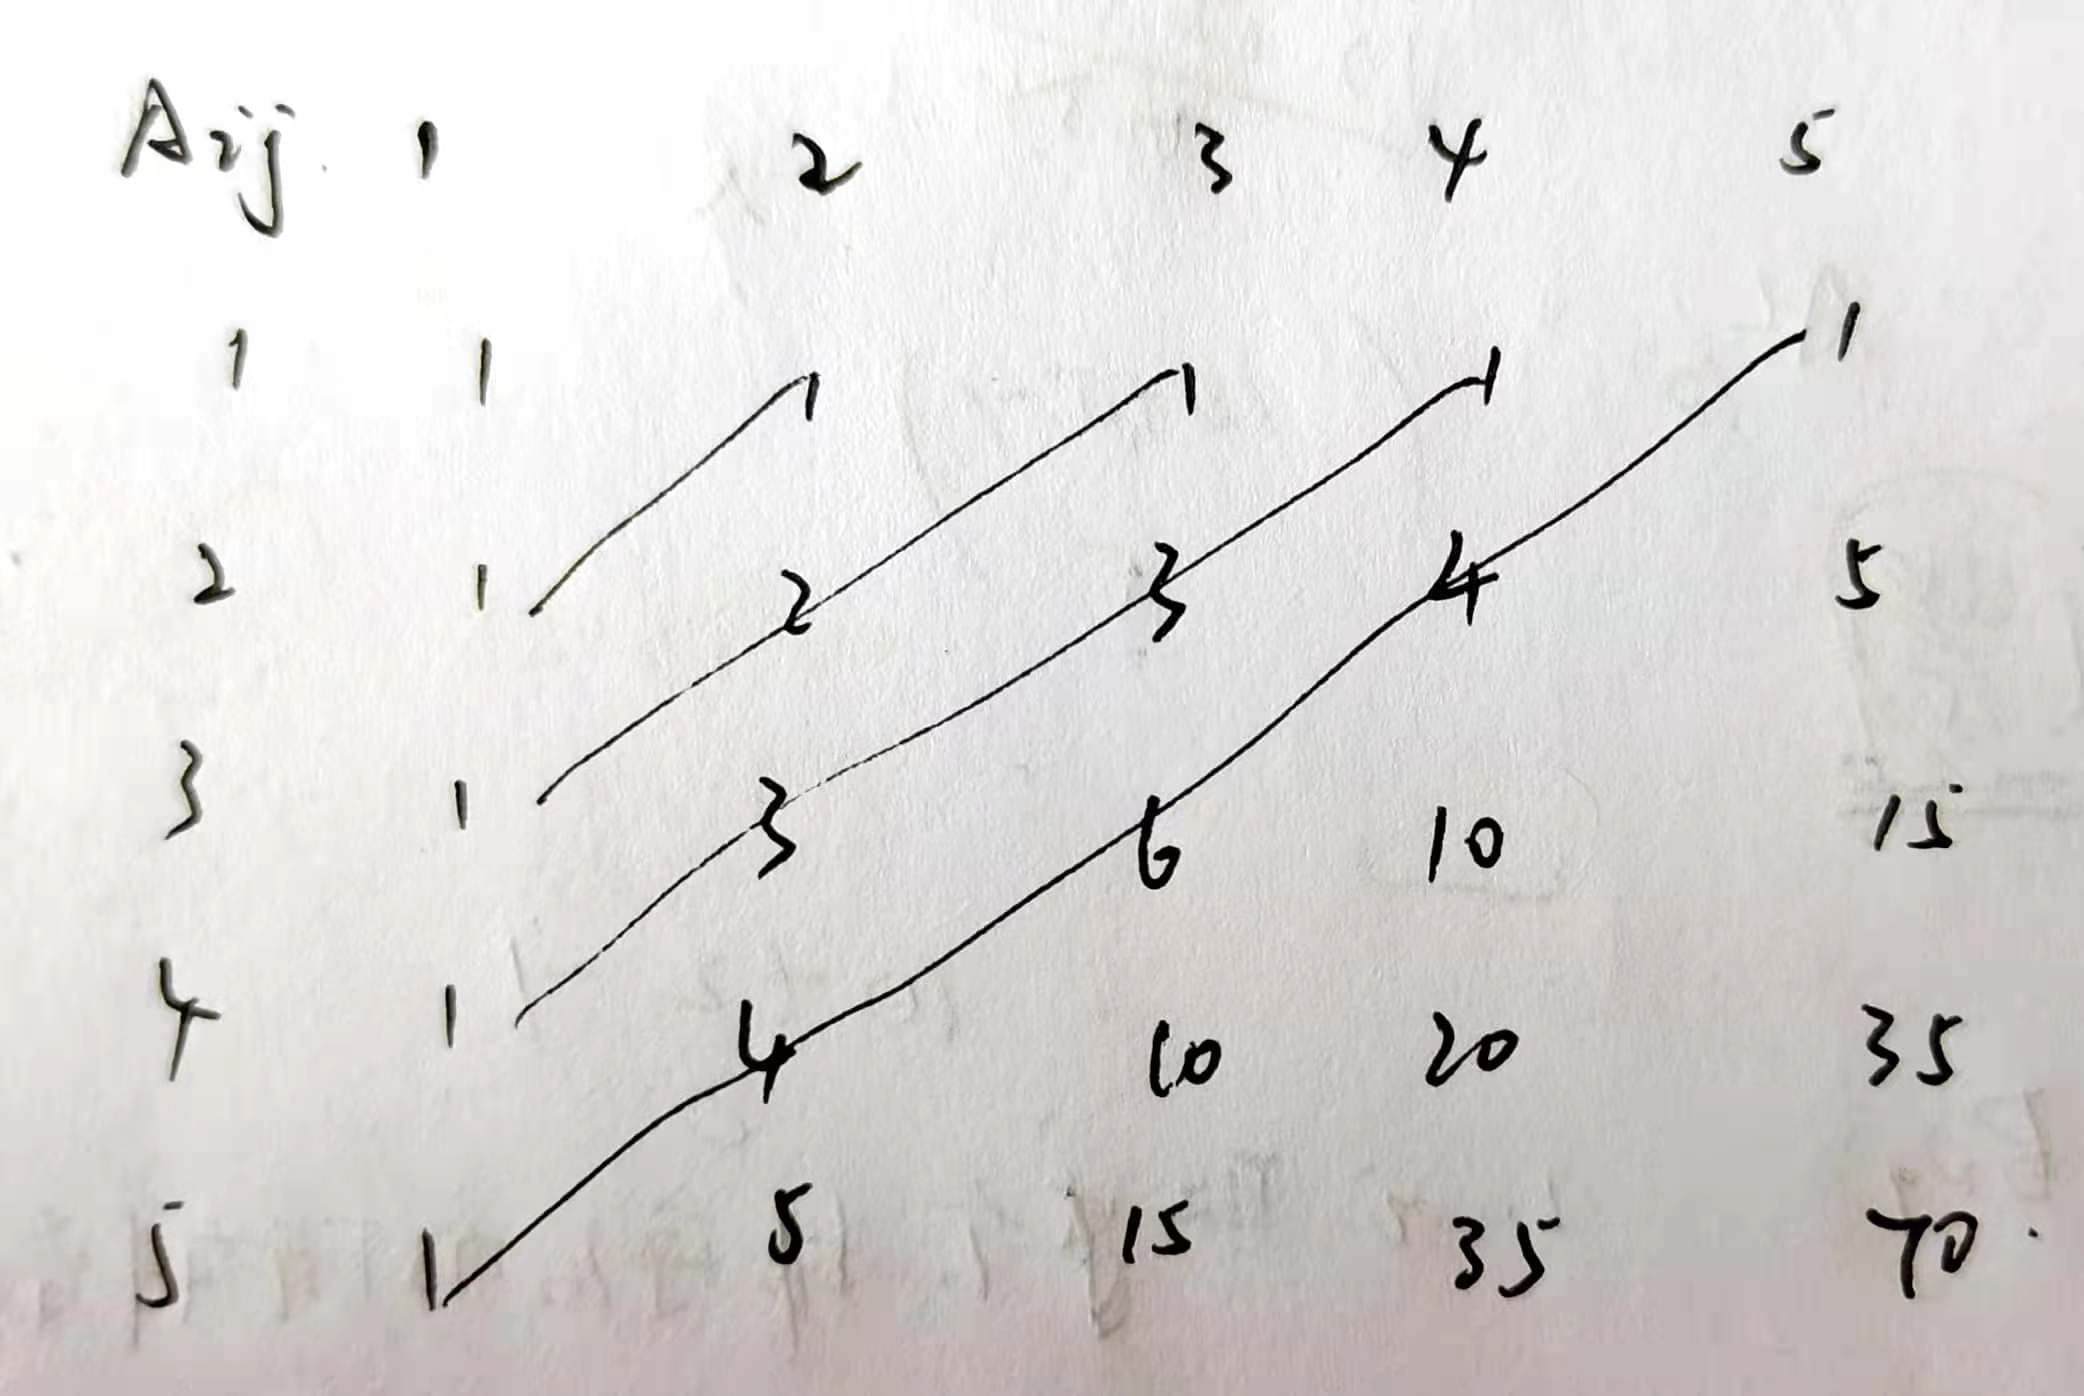
\includegraphics[width=0.5\textwidth]{figure.jpg}
    }
    可以发现$|A_{ij}|$构成了从左上角开始的一个杨辉三角,则$|A_{ij}| = \binom{i+j-2}{j-1}$,于是
    \begin{equation*}
        \begin{aligned}
            |B_{ij}| =&\ |A_{1j}|+|A_{2j}| +\cdots +|A_{ij}| = \binom{j-1}{j-1}+\binom{j}{j-1}+\cdots+\binom{i+j-2}{j-1}\\
            \xlongequal{\text{hockey stick identity}}&\ \binom{i+j-1}{j}
        \end{aligned}
    \end{equation*}
    所以,总样本空间$|\Omega| = |B_{10,5}| = \binom{14}{5}$,且可以直接给出$(X_i=j)$的表达式,由于第$i$位要求为$j$,将整个序列分为$X_1\cdots X_{i-1}$和$X_i\cdots X_5$两段,第一段没有对开头元素的限制,所以有$|B_{j,i-1}|$种排法,第二段要求开头元素为$i$,所以有$|A_{11-j,6-i}|$种排法,故$|(X_i=j)| = |B_{j,i-1}|\cdot|A_{11-j,6-i}|=\binom{15-i-j}{5-i}\binom{i+j-2}{i-1}$,于是$X_i$的分布律为
    \begin{equation*}
        \begin{aligned}
            \left(\begin{matrix}
                1&2&3&4&5&&\\
                \frac{\binom{14-i}{5-i}\binom{i-1}{i-1}}{\binom{14}{5}}&\frac{\binom{13-i}{5-i}\binom{i}{i-1}}{\binom{14}{5}}&\frac{\binom{12-i}{5-i}\binom{i+1}{i-1}}{\binom{14}{5}}&\frac{\binom{11-i}{5-i}\binom{i+2}{i-1}}{\binom{14}{5}}&\frac{\binom{10-i}{5-i}\binom{i+3}{i-1}}{\binom{14}{5}}&&\\
                &&6&7&8&9&10\\
                &&\frac{\binom{9-i}{5-i}\binom{i+4}{i-1}}{\binom{14}{5}}&\frac{\binom{8-i}{5-i}\binom{i+5}{i-1}}{\binom{14}{5}}&\frac{\binom{7-i}{5-i}\binom{i+6}{i-1}}{\binom{14}{5}}&\frac{\binom{6-i}{5-i}\binom{i+7}{i-1}}{\binom{14}{5}}&\frac{\binom{5-i}{5-i}\binom{i+8}{i-1}}{\binom{14}{5}}
            \end{matrix}\right)
        \end{aligned}
    \end{equation*}
    代入$i=1,3,5$即可得到$X_1,X_3,X_5$对应的分布律。

\end{solution}
\paragraph{习题3.2}
\paragraph{2.}求$n$次独立重复的$\text{Bernoulli}$试验中成功奇数次的概率$p_n$。
\begin{proof}
    设$X$服从参数$n, p$的二项分布,$p$为$\text{Bernoulli}$试验中成功的概率,即$X\sim B(n, p)$,则
    \begin{equation*}
        \begin{aligned}
            p_n = \sum_{k=1}^{[(n+1)/2]}\binom{n}{2k-1}p^{2k-1}q^{n-2k+1}
        \end{aligned}
    \end{equation*}
    其中$[x],\ (x\in\mathbb{R})$为向下取整符号。
\end{proof}
\paragraph{5.}将$[0,1]$上的均匀分布推广到有限区间$[a,b]$上,写出其分布函数。
\begin{solution}
    设$F(x) = U[0,1]$,做线性变换$\varphi(x) = (b-a)x+a$,则
    \begin{equation*}
        G(x) = F(\varphi(x)) = 
        \begin{cases}
            0, &\quad x\leqslant a,\\
            \dfrac{x-a}{b-a},&\quad a<x\leqslant b,\\
            1,&\quad x > b.
        \end{cases}
    \end{equation*}
    为$[a,b]$上的均匀分布。
\end{solution}
\paragraph{10.}两名篮球队员轮流投篮,直至某人投中为止,如果甲投中的概率为$0.4$,乙投中的概率为$0.6$,现在让甲先投,求两球员投篮次数的分布律。
\begin{solution}
    设随机变量$X$表示两球员的投篮总次数,每一次投篮中甲、乙投不中的概率分别记为$q_1,q_2$,投中的概率分别为$p_1,p_2$,则该问题可转化为参数为$q_1,q_2$和$n$的几何分布问题,则
    \begin{equation*}
        \begin{aligned}
            \mathbf{P}(X = x)=&\  
            \begin{cases}
                \binom{2k}{k}q_1^kq_2^kp_1,&\quad x = 2k+1,\ (k = 0, 1,\cdots),\\
                \binom{2k-1}{k}q_1^kq_2^{k-1}p_2,&\quad x = 2k,\ (k=1, 2,\cdots).\\
            \end{cases}\\
            \xlongequal{\text{代入数值}}&\ \begin{cases}
                \binom{2k}{k}(0.6)^k(0.4)^{k+1},&\quad x = 2k+1,\ (k = 0, 1,\cdots),\\
                \binom{2k-1}{k}(0.6)^{k+1}(0.4)^{k-1},&\quad x = 2k,\ (k=1, 2,\cdots).\\
            \end{cases}
        \end{aligned}
    \end{equation*}
\end{solution}
\paragraph{12.}设某汽车站在一天的某段时间中有$1000$辆汽车通过,每辆汽车在该段时间出事故的概率为$0.0001$,求该段时间出事故的汽车数不小于$2$的概率。
\begin{solution}
    设$n = 1000, p = 0.0001$,$X\sim B(n, p)$,则
    \begin{equation*}
        \begin{aligned}
            \mathbf{X\geqslant 2} =&\ 1-\mathbf{X \leqslant 1} \\
            =&\ 1-\mathbf{X=  0}-\mathbf{X=1}\\
            =&\ 1 - (1-p)^{1000}-\binom{1000}{1}p(1-p)^{999}\\
            \approx&\ 0.00467
        \end{aligned}
    \end{equation*}
\end{solution}
\paragraph{14.}有甲、乙两种酒各$4$杯,如果从$8$杯中挑$4$杯,能将甲种酒挑出来,叫做试验成功一次。(1) 某人随机地去挑,求试验成功一次的概率;(2) 某人独立试验$10$次,成功了$3$次,问:他是猜对的,还是他确有鉴别能力?
\begin{solution}
    (1) 设事件$A$为一次试验成功,$\Omega$为一次试验的全部情况,则
    \begin{equation*}
        \mathbf{P}(A) = \frac{|A|}{|\Omega|} = \frac{\binom{4}{4}}{\binom{8}{4}} = \frac{1}{70}
    \end{equation*}

    (2) 设$n=10, p = \mathbf{P}(A)$,$X\sim B(n, p)$,则
    \begin{equation*}
        \mathbf{P}(X = 3) = \binom{10}{3}\left(\frac{1}{70}\right)^3\left(\frac{69}{70}\right)^7 \approx 0.00032 < 0.001
    \end{equation*}
    由于$\mathbf{P}(X=3)$为小概率事件,所以可以认为他有鉴别能力。
\end{solution}
\paragraph{习题3.3}
\paragraph{3.}分子运动速度的绝对值$X$服从$\text{Maxwell}$分布,有概率密度函数
\begin{equation*}
    p(x)=ax^2\exp\left\{-\frac{x^2}{b}\right\},\quad x > 0,
\end{equation*}
其中$b>0$是已知常数,$a$是待定常数。求$a$。
\def\P{\mathbf{P}} % 一个简单的宏定义
\begin{solution}
    由题可得
    \begin{equation*}
        \begin{aligned}
            \int_{-\infty}^{+\infty}p(x)\,dx =&\ \int_{-\infty}^{+\infty}ax^2e^{-x^2/b}\,dx=-\frac{ab}{2}\int_{-\infty}^{+\infty}x\,d(e^{-x^2/b})\\
            =&\ \frac{ab}{2}\int_{-\infty}^{+\infty}e^{-x^2/b}\,dx=\frac{ab}{2}\sqrt{\pi b} = 1
        \end{aligned}
    \end{equation*}
    所以
    \begin{equation*}
        a = \frac{2}{b\sqrt{\pi b}}
    \end{equation*}
\end{solution}
\paragraph{4.}已知随机变量$X$的密度函数为
\begin{equation*}
    p(x)=\begin{cases}
        x,\quad&0<x\leqslant 1,\\
        2-x,\quad&1<x\leqslant 2,
    \end{cases}
\end{equation*}
试求:(1) $X$的分布函数;(2) 概率$\P(0.2<x<1.3)$。

\begin{solution}
    (1). 由题可得\begin{equation*}
        F(x) = \P(X\leqslant x) = \int_{-\infty}^xp(x)\,dx=\begin{cases}
            \frac{1}{2}x^2,\quad&0< x\leqslant 1\\
            -\frac{1}{2}x^2+2x-1,\quad&1<x\leqslant 2
        \end{cases}
    \end{equation*}

    (2). 由(1)可知 \begin{equation*}
        \P(0.2<X<1.3)=F(1.3)-F(0.2) = -\frac{1}{2}(1.3)^2+2\cdot 1.3-1-\frac{1}{2}(0.2)^2=0.757
    \end{equation*}
\end{solution}

\paragraph{6.}设$p(x) = e^{-e(x-a)},\quad x > 0.$ (1) 求$a$使$p(x)$为密度函数;(2) 若随机变量$X$以此$p(x)$为密度,求$b$使$\P(X>b) = b.$
\begin{solution}
    (1). 由于$p(x)$为密度函数,则有
    \begin{equation*}
        \begin{aligned}
            &\ \int_0^{+\infty}e^{-e(x-a)}\,dx = -\frac{1}{e}e^{-e(x-a)}\biggl|_0^{+\infty}=\frac{1}{e}e^{ea} = 1\\
            \Rightarrow&\ a = \frac{1}{e}
        \end{aligned}
    \end{equation*}

    (2). 由(1)可知,$p(x) = e^{-ex+1}$,则
    \begin{equation*}
        \begin{aligned}
            &\ \P(X>b) = \int_b^{+\infty}e^{-ex+1}\,dx = \frac{1}{e}e^{-eb+1} = b\\
            \Rightarrow&\ e^{-eb+1} = eb\Rightarrow eb = 1\Rightarrow b = \frac{1}{e}
        \end{aligned}
    \end{equation*}
\end{solution}
\paragraph{7.}设连续性随机变量$X$的分布函数在区间$[0,1]$中严格单调,$\P(X\leqslant 0.29)=0.75$,$Y=1-X$,求实数$x$,使$\P(Y\leqslant x) = 0.25$。
\begin{solution}
    \begin{equation*}
        \P(Y\leqslant x) = \P(1-X\leqslant x) = \P(X\geqslant 1-x) = 0.25
    \end{equation*}
    由于$\P(X\leqslant 0.29)=0.75$,则$\P(X\geqslant 0.29)=0.25$,又由于$X$的分布函数的严格单调性,知$1-x=0.29$,所以$x = 0.71$。
\end{solution}
\paragraph{9.}设\begin{equation*}
    F(x)=\begin{cases}
        0,\quad&x<0,\\
        \frac{1}{3}(1+2x),\quad&0\leqslant x < 1,\\
        1,\quad&x \geqslant 1.
    \end{cases}
\end{equation*}
证明:(1) $F(x)$是一个分布函数;(2) $F(x)$既不是离散型的也不是连续型的,但它可以写为这两种类型分布函数的线性组合。
\begin{proof}
    (1). 通过$F(x)$的定义式,不难得出$F(x)$具有非降性,规范性,由于$F(x)$只有在$x=0$处间断,所以考虑该点的右连续性
    \begin{equation*}
        \lim_{t\downarrow 0}F(t) = \lim_{t\downarrow 0}\frac{1}{3}(1+2x)=\frac{1}{3} = F(0)
    \end{equation*}
    则$F(x)$满足右连续性。综上,$F(x)$是一个分布函数。

    (2). 由于$F(x)$不是阶梯型函数,所以$F(x)$不是离散型的,又由于$F(x)$在$x=\frac{1}{3}$处间断,所以$F(x)$也不是连续型的。设$F_1(x)$为$U[0,1]$对应的连续型分布函数,$F_2(x)$为分布律为$\P(x = 0) = 1$的离散型分布函数,则$F(x)$可以表示为$F_1(x),F_2(x)$的凸组合
    \begin{equation*}
        F(x) = \frac{2}{3}F_1(x) +\frac{1}{3}F_2(x)
    \end{equation*}
\end{proof}
\paragraph{习题 3.4}
\paragraph{1.}某电话交换台每分钟收到的呼唤次数服从参数为$4$的$\text{Poisson}$分布。(1) 求每分钟恰有$8$次呼唤的概率;(2) 求每分钟的呼唤次数大于$10$的概率。
\begin{solution}
    (1) $\P_1=  p(8; 4) = \dfrac{4^8}{8!}e^{-4} \approx 0.02977$

    (2) $\P_2 = \displaystyle\sum_{k=11}^{+\infty}p(k;4) = 1-\sum_{k=0}^{10}\frac{4^k}{k!}e^{-4} \approx 0.002839766$
\end{solution}
\paragraph{4.}在某$63$年中,某地的夏季($5\sim 9$月)共有$180$天下暴雨,求一个夏季中下暴雨不超过$4$天的概率。
\begin{solution}
    平均$1$年夏季下暴雨天数为:$\frac{180}{63}=\frac{20}{7}$,由于每一天下是否下暴雨是相互独立地,可以近似认为是满足$\lambda = \frac{20}{7}$的$\text{Poisson}$分布,所以,一个夏季中下暴雨不超过$4$天的概率为:
    \begin{equation*}
        \P = \sum_{k=0}^4p(k;\frac{20}{7}) = \sum_{k=0}^4\frac{\left(\frac{20}{7}\right)^k}{k!}e^{-20/7} \approx 0.838669
    \end{equation*}
\end{solution}
\paragraph{7.}保险公司的资料表明,持某种人寿保险单的人在保险期内死亡的概率为$0.005$。现出售这种保单$1200$份,求保险公司至多赔付$10$份的概率。
\begin{solution}
    设出售$1200$份保单要赔付随机变量$X$份,由于每个人的死亡为独立事件,所以满足二项分布,即$X\sim B(1200, 0.005)$,由于$n$较大,且$p$较小,所以可以近似视为参数为$1200\times 0.005 = 6$的$\text{Poisson}$分布,则
    \begin{equation*}
        \P = \sum_{k=0}^{10}b(k;1200,0.005)\approx\sum_{k=0}^{10}p(k;6) = \sum_{k=0}^{10}\frac{6^k}{k!}e^{-6} = 0.957379
    \end{equation*}
\end{solution}
\paragraph{12.}通过一交叉路口的汽车流可以看作一个$\text{Poisson}$过程。如果$1$分钟内没有汽车通过的概率是$0.02$,求$2$分钟内有多于$1$辆汽车通过的概率。
\begin{solution}
    设$X_t$为在$t$分钟以前通过交叉路口的汽车数目,则$X_t$可以视为一个$\text{Poisson}$分布,则$1$分钟没有汽车通过的概率可以表示为
    \begin{equation*}
        \P(x_1 = 0) = e^{-\lambda} = 0.02
    \end{equation*}
    所以$2$分钟内有多于$1$辆车通过的概率为
    \begin{equation*}
        \P = 1- \P(x_2 = 0) = 1-e^{-2\lambda} = 1-(0.02)^2 = 0.9996
    \end{equation*}
\end{solution}
\paragraph{15.}证明非负值随机变量$X$服从指数分布的充分必要条件是它是无记忆性的,即\begin{equation*}
    \P\{X>s+t|X>s\}=\P\{X>t\},\quad\forall s,t > 0.
\end{equation*}

\begin{proof}
    “$\Rightarrow$”:设随机变量$X$服从指数分布,则$\P(X>x) = e^{-\lambda x}$,
    \begin{equation*}
        \P(X>s+t|X>s) = \frac{\P(X>s+t)}{\P(X>s)} = \frac{e^{-\lambda(s+t)}}{e^{-\lambda s}} = e^{-\lambda t} = \P(X > t)
    \end{equation*}
    
    “$\Leftarrow$”:对于$\forall s, t > 0$,有$\P(X>s+t) = \P(X>s)\cdot \P(X>t)$,令$f(x) = \P(X>x)$,则
    \begin{equation*}
        f(s+t) = f(x)\cdot f(t)
    \end{equation*}
    对$\forall x \in \mathbb{R}_{\geqslant 0}$,则$f(x)=f(x+0) = f(x)\cdot f(0)$,若$f(x)\equiv 0$,则与$X$为随机变量,矛盾。所以$\exists f(x)\neq 0$,则$f(0) = 1$。
    
    令$f(1) = a$,对于任意的有理数$x\in\mathbb{Q}, x=  \frac{p}{q}$,其中$p,q$互素,则
    \begin{equation*}
        \begin{aligned}
            &\ \left(f(x)\right)^q = \left(f(\frac{p}{q})\right)^q = f(\frac{p}{q}\cdot q) = f(p) = f(1\cdot p) = \left(f(1)\right)^p = a^p\\
            \Rightarrow&\ f(x) = a^{p/q} = a^x
        \end{aligned}
    \end{equation*}
    对任意的无理数$x\in\mathbb{R}-\mathbb{Q}$,由于$\lim\limits_{n\rightarrow \infty}\frac{[nx]}{n} = x$且$f\left(\frac{[nx]}{n}\right) = a^{[nx]/n}$,当$n\rightarrow\infty$时,由$f(x)$的连续性可知,得$f(x) = a^x$。

    所以,$x\in \mathbb{R}_{\geqslant 0}$,都有$f(x) = a^x$,不妨令$a = e^{-\lambda}$,则$f(x) = e^{-\lambda x}$,满足指数分布。

\end{proof}
\paragraph{习题 3.5}
\paragraph{2.}若$X$的分布函数为$\mathcal{N}(60,9)$,求分点$x_1,x_2,x_3,x_4$使$X$若在区间\begin{equation*}
    (-\infty, x_1),\ (x_1,x_2),\ (x_2, x_3),\ (x_3, x_4),\ (x_4,\infty)
\end{equation*}
中的概率之比为$7:24:38:24:7.$
\begin{solution}
    令$Z = \frac{X - 60}{3}$,则$Z\sim \mathcal{N}(0,1)$,由正态分布的性质可知
    \begin{equation*}
        \begin{aligned}
            &\P(Z\leqslant z_4) = 1-\frac{7}{100} = 0.93 \approx 1.48\Rightarrow x_4 = 3z_4+60 = 64.44\\
            &\P(Z\leqslant z_3) = 1-\frac{24+7}{100} = 0.69\approx 0.5\Rightarrow x_3 = 3z_3+60 = 61.5
        \end{aligned}
    \end{equation*}
    由正态分布的对称性可知:$x_2 = 58.5, x_1 = 55.56$。
\end{solution}
\paragraph{4.}假定随机变量$X$只取区间$(0,1)$中的值,且对任何$0<x<y<1$,$X$落在子区间$(x,y)$内的概率仅与$y-x$有关。证明:$X$服从$U(0,1)$(即区间$(0,1)$上的均匀分布)。
\begin{proof}
    对$\forall 0<x<y<1,\ z = y-x$,根据题意知,存在$f(z)$,使得$\displaystyle \int_x^yp(t)\,dt = f(y-x)$,两侧同时对$y$求导,可得$p(y) = f'(y-x)$,令$y=1$,由于$x$的任意性,$\forall z\in (0,1)$,都有$f'(z) = p(1)$,则$p(y) = f'(y-x) = p(1)$,又由于
    \begin{equation*}
        1=\P(0<X<1)=\int_0^1p(1)\,dt = p(1)
    \end{equation*}
    则$p(x) = 1\ (x\in (0,1))$,服从$U(0,1)$均匀分布。
\end{proof}
\paragraph{8.}某公司生产的电子管的寿命$X$(以小时计)服从正态分布$\mathcal{N}(160,\sigma^2)$,为了达到要求\newline$\P(120<X\leqslant 200)\geqslant 0.80$,试问,$\sigma$的最大可能值是多少?
\begin{solution}
    设$X\sim \mathcal{N}(160,\sigma^2)$,$\P(120<X\leqslant 200)\geqslant 0.8$,由正态分布的对称性可知,$\P(X\leqslant 200) = 0.9$,通过查表可知$\dfrac{200-160}{\sigma}\geqslant 1.28$,则$\sigma \leqslant \dfrac{200-160}{1.28} = 31.25$,所以$\sigma$的最大可能值约为$31.25$。
\end{solution}
\paragraph{9.}设随机变量$X$服从$\mathcal{N}(0,1)$,$Y=X$或$-X$,视$|X|\leqslant 1$或$|X|>1$而定。求$Y$的分布。
\begin{solution}
    根据题意可知,且标准正态分布的分布函数满足$\Phi(-x) = 1-\Phi(x)$,所以
    \begin{equation*}
        Y = 
        \begin{cases}
            X,\quad&|X|\leqslant 1,\\
            -X,\quad&|X| > 1.
        \end{cases}
        \quad\Rightarrow
        F_Y(x) = \begin{cases}
            \Phi(x),\quad&|x|\leqslant 1,\\
            1-\Phi(x),\quad&|x| > 1.
        \end{cases}
    \end{equation*}
\end{solution}
\paragraph{习题 3.6}
\def\disp{\displaystyle}
\paragraph{1.}设离散型随机变量$X$的分布律为
\begin{equation*}
    \P(X=0)=\frac{1}{4},\quad\P(X=\frac{\pi}{2})=\frac{1}{2},\quad\P(X=\pi)=\frac{1}{4}.
\end{equation*}
求$\disp\frac{2}{3}X+2$及$\disp\cos X$的分布律。
\begin{solution}
    \begin{equation*}
        (\frac{2}{3}X+2)\sim\left(\begin{matrix}
            2&\frac{\pi}{3}+2&\frac{2}{3}\pi+2\\
            \frac{1}{4}&\frac{1}{2}&\frac{1}{4}
        \end{matrix}\right),\quad
        \cos X\sim\left(\begin{matrix}
            1&0&-1\\
            \frac{1}{4}&\frac{1}{2}&\frac{1}{4}
        \end{matrix}\right)
    \end{equation*}
\end{solution}
\paragraph{3.}设$\disp X\sim U\left[-\frac{\pi}{2},\frac{\pi}{2}\right]$,求$Y=\cos X$的分布函数。
\begin{solution}
(i) $x<0$,$\P(Y\leqslant X) = 0$;

(ii) $0\leqslant X < 1$,$\disp\P(Y\leqslant X) = \P(X \leqslant -\arccos x) + \P(X > \arccos x) = 1-\frac{2}{\pi}\arccos x$;

(iii) $X\geqslant 1$,$\P(Y \leqslant X) = 1$。

综上\begin{equation*}
    F_Y(x) = \begin{cases}
        0,&\quad x < 0,\\
        1-\frac{2}{\pi}\arccos x,&\quad 0\leqslant x < 1,\\
        1,&\quad x \geqslant 1.
    \end{cases}
\end{equation*}
\end{solution}
\paragraph{5.}设$X\sim U(-2,3)$,\begin{equation*}
    Y = \begin{cases}
        -1,&\quad X\leqslant -1,\\
        X,&\quad -1<X<1,\\
        1,&\quad X \geqslant 1,
    \end{cases}
\end{equation*}
分别求$Y$和$Y^{-2}$的分布函数。
\begin{solution}
    (i) $x < -1$,$\P(Y\leqslant x) = 0$;

    (ii) $-1\leqslant x\leqslant 1$,$\disp\P(Y\leqslant x) = \P(X\leqslant x) = \frac{1}{5}x+\frac{2}{5}$;

    (iii) $X > 1$,$\P(Y\leqslant x) = 1$。

    综上
    \begin{equation*}
        F_Y(x) = \begin{cases}
            0,&\quad x < -1\\
            \frac{1}{5}x+\frac{2}{5},&\quad -1\leqslant x\leqslant 1\\
            1,&\quad x > 1
        \end{cases}
    \end{equation*}

    (i) $x<1$,$\P(Y^2\leqslant x) = 0$;

    (ii) $x\geqslant 1$,$\disp\P(Y^2\leqslant x) = \P(|X|\geqslant \frac{1}{\sqrt{x}}) = 1-\left(\frac{1}{5\sqrt{x}}+\frac{2}{5}\right)+\left(\-\frac{1}{5\sqrt{x}}+\frac{2}{5}\right) = 1-\frac{2}{5\sqrt{x}}$。

    综上
    \begin{equation*}
        F_{Y^2}(x) = \begin{cases}
            0,&\quad x < 1\\
            1-\frac{2}{5\sqrt{x}},&\quad x \geqslant 1
        \end{cases}
    \end{equation*}
\end{solution}
\paragraph{7.}设$X\sim\mathcal{N}(0,1)$,分别求$e^X,1/X^2,2X^2+1$和$|X|$的概率密度函数。
\begin{solution}设$X$对应的密度函数为$\disp p(x) = \frac{1}{\sqrt{2\pi}}e^{-\frac{x^2}{2}}$,所求的密度函数分别记为$p_i\ (i=1,2,3,4)$,则
    \begin{equation*}
        \begin{aligned}
            &(1)\ p_1(x) = p(\log |x|)\frac{1}{|x|} = \frac{1}{\sqrt{2\pi}|x|}e^{\frac{-\log^2|x|}{2}};\\
            &(2)\ p_2(x) = p(|x|^{-\frac{1}{2}})(\frac{1}{2}|x|^{-\frac{3}{2}}) = \frac{1}{2\sqrt{2\pi}|x|^{-\frac{3}{2}}}e^{-\frac{1}{2|x|}};\\
            &(3)\ p_3(x) = p(\frac{\sqrt{|x-1|}}{2})\frac{1}{4\sqrt{|x-1|}} = \frac{1}{4\sqrt{2\pi|x-1|}}e^{-\frac{|x-1|}{8}};\\
            &(4)\ p_4(x) = p(|x|) = \frac{1}{\sqrt{2\pi}}e^{-\frac{x^2}{2}}.
        \end{aligned}
    \end{equation*}
\end{solution}

\paragraph{10.}设随机变量$X$具有密度函数$p_X(x)$,并设
\begin{equation*}
    \begin{aligned}
        (1)\ g_1(x) = \begin{cases}
            1,&\quad x > 0,\\
            -1,&\quad x \leqslant 0;
        \end{cases}\quad (2)\ g_2(x)=\begin{cases}
            x,&\quad |x|\geqslant b,\\
            0,&\quad |x| <b;
        \end{cases}\quad
        (3)\ g_3(x)=\begin{cases}
            b,&\quad x \geqslant b,\\
            x,&\quad |x| < b,\\
            -b,&\quad x\leqslant -b.
        \end{cases}
    \end{aligned}
\end{equation*}
求$Y=g_i(X)$的分布,$i=1,2,3$。
\begin{solution}
    (1). (i) $x < -1$,$\P(Y\leqslant x) = 0$;

    (ii) $-1\leqslant x < 1$,$\disp\P(Y\leqslant x) = \P(X \leqslant 0) = \int_{-\infty}^x\P_X(\xi)\,d\xi$;

    (iii) $x\geqslant 1$,$\disp \P(Y\leqslant x) = 1$.

    综上
    \begin{equation*}
        F_{g_1(X)} = \begin{cases}
            0,&\quad x < -1,\\
            \int_{-\infty}^x\P_X(\xi)\,d\xi,&\quad -1\leqslant x < 1,\\
            1,&\quad x\geqslant 1.
        \end{cases}
    \end{equation*}

    (2). (i) $x\leqslant -b$,$\disp\P(Y\leqslant x) = \P(X\leqslant x)=\int_{-\infty}^x\P_X(\xi)\,d\xi$;

    (ii) $-b\leqslant x < 0$,$\disp\P(Y\leqslant x) = \P(X\leqslant -b) = \int_{-\infty}^{-b}\P_X(\xi)\,d\xi$;

    (iii) $0\leqslant x < b$,$\disp\P(Y\leqslant x)=\P(X\leqslant b)=\int_{-\infty}^b\P_X(\xi)\,d\xi$;

    (iv) $b\leqslant x$,$\disp\P(Y\leqslant x) = \P(X < x) = \int_{-\infty}^x\P_X(\xi)\,d\xi$.

    综上
    \begin{equation*}
        \P_{g_2(X)} = \begin{cases}
            \int_{-\infty}^x\P_X(\xi)\,d\xi,&\quad |x|\geqslant b,\\
            \int_{-\infty}^{-b}\P_X(\xi)\,d\xi,&\quad -b< x < 0,\\
            \int_{-\infty}^{b}\P_X(\xi)\,d\xi,&\quad 0\leqslant x < b.\\
        \end{cases}
    \end{equation*}

    (3). (i) $x < -b$,$\P(Y\leqslant x) = 0$;

    (ii) $-b\leqslant x  < b$,$\disp\P(Y\leqslant x) = \P(X\leqslant x) = \int_{-\infty}^x\P_X(\xi)\,d\xi$;

    (iii) $b\leqslant x$,$\disp \P(Y\leqslant x) = 1$.
    
    综上
    \begin{equation*}
        F_{g_3(X)} = \begin{cases}
            0,&\quad x< -b\\
            \int_{-\infty}^x\P_X(\xi)\,d\xi,&\quad -b\leqslant x < b\\
            1,&\quad b\leqslant x.
        \end{cases}
    \end{equation*}
\end{solution}

\iffalse
% 图片模板
\centerline{
    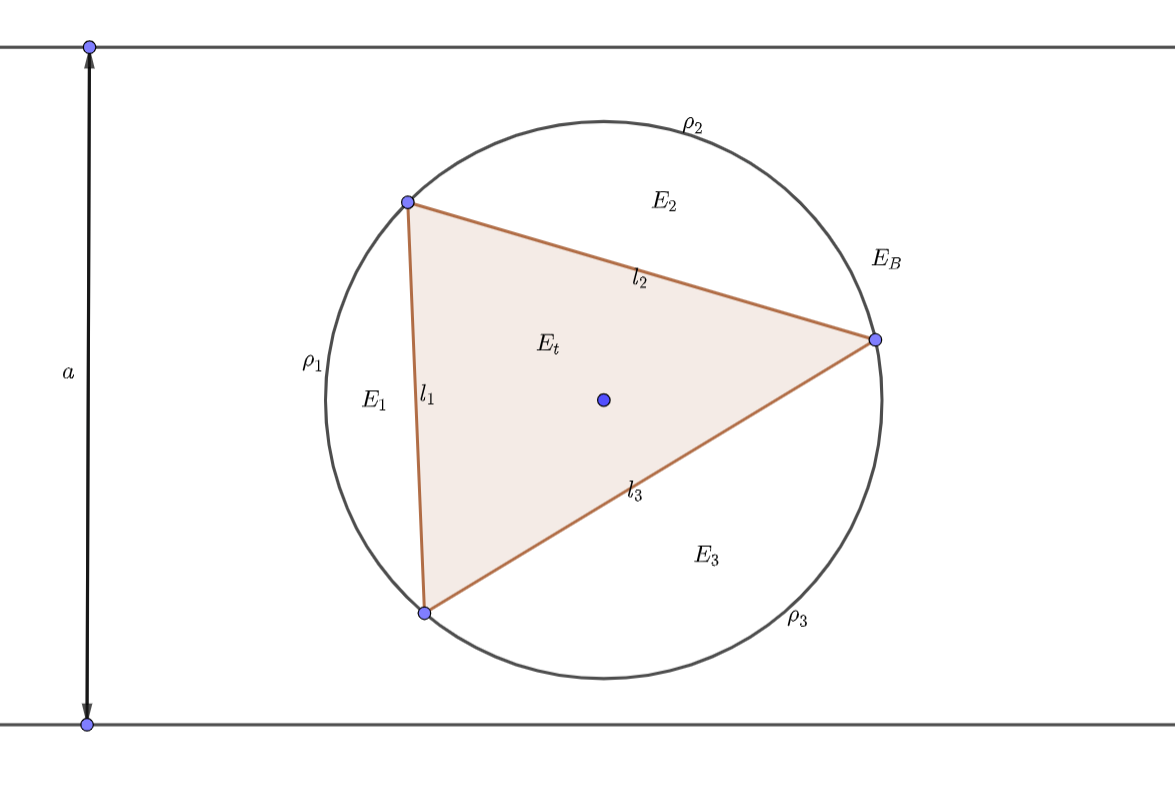
\includegraphics[width=0.8\textwidth]{figure.png}
}
\fi
\iffalse
% 表格模板
\renewcommand\arraystretch{0.8} % 设置表格高度为原来的0.8倍
\begin{table}[!htbp] % table标准
    \centering % 表格居中
    \begin{tabular}{p{1cm}<{\centering}p{1cm}<{\centering}p{3cm}<{\centering}p{5cm}<{\centering}} % 设置表格宽度
    %\begin{tabular}{cccc}
        \toprule
        $x_i$ & $f[x_1]$ & $f[x_i,x_{i+1}]$ & $f[x_i,x_{i+1},x_{i+2}]$ \\
        \midrule
        $x_0$ & $f(x_0)$ &                  &                          \\
        $x_0$ & $f(x_0)$ & $f'(x_0)$        &                          \\
        $x_0$ & $f(x_1)$ & $\frac{f(x_1)-f(x_0)}{x_1-x_0}$ & $\frac{f(x_1)-f(x_0)}{(x_1-x_0)^2}-\frac{f'(x_0)}{x_1-x_0}$\\
        \bottomrule
    \end{tabular}
\end{table}

\def\Log{\text{Log}} % 一个简单的宏定义
$\Log$ % 调用方法
\fi

\end{document}